% use paper, or submit
% use 11 pt (preferred), 12 pt, or 10 pt only

\documentclass[letterpaper, preprint, paper,11pt]{AAS}	% for preprint proceedings
%\documentclass[letterpaper, paper,11pt]{AAS}		% for final proceedings (20-page limit)
%\documentclass[letterpaper, paper,12pt]{AAS}		% for final proceedings (20-page limit)
%\documentclass[letterpaper, paper,10pt]{AAS}		% for final proceedings (20-page limit)
%\documentclass[letterpaper, submit]{AAS}			% to submit to JAS

\usepackage{bm}
\usepackage{amsmath}
\usepackage{subfigure}
%\usepackage[notref,notcite]{showkeys}  % use this to temporarily show labels
\usepackage[colorlinks=true, pdfstartview=FitV, linkcolor=black, citecolor= black, urlcolor= black]{hyperref}
\usepackage{overcite}
\usepackage{footnpag}			      	% make footnote symbols restart on each page

% Added packages 2019 Feb 17
\usepackage{float}
\usepackage{amssymb}
%\usepackage{graphicx} % Allows including images
%\usepackage{mathrsfs}
\usepackage{booktabs} % Allows the use of \toprule, \midrule and \bottomrule in tables


\begin{document}
	
	\title{SUN-AVOIDANCE SLEW PLANNING ALGORITHM WITH POINTING AND ACTUATOR CONSTRAINTS}
	
	\author{
		Mohammad Ayoubi\thanks{Title, department, affiliation, postal address.} and Junette Hsin\thanks{Title, department, affiliation, postal address.}
	}
	
	
	\maketitle{} 		
	
	
	\begin{abstract}
		
		A sun avoidance slew maneuver is described in this paper. The algorithm finds the angular velocity, angular acceleration, and quaternion profiles needed to avoid the sun vector that lies near the plane of a sensor's FOV onboard a spacecraft. 
		
		% The abstract should briefly state the purpose of the manuscript, the problem to be addressed, the approach taken, and the nature of results or conclusions that can be expected. It should stand independently and tell enough about the manuscript to permit the reader to decide whether the subject is of specific interest. The abstract shall be typed single space, justified, centered, and with a column width of 4.5 inches. The abstract is not preceded by a heading of ``Abstract'' and its length may not extend beyond the first page.
		
	\end{abstract}
	
	\section{Simulation}
				
		A simulation is shown in the following figures. The initial, final, and sun position vectors were randomized for each run. 
		
		$\phi_1$, $\phi_2$, and $\phi_3$ were found using the methods discussed in the algorithm description. Several intermediate frames had to be calculated for the simulation to run. In addition to the slew plane, a sun-to-position frame was constructed in order to calculate the path that the spacecraft takes around the sun vector. SP This path had to be traced by rotating the vector that connects the sun and $P_1$ vectors, which is the green line on the right in the figure below and will be called $V$. $V$ was rotated from $P_1$ to $P_2$ by angle $\phi_2$. 
		
			\begin{figure}[H]
				\label{fig:phi2_geometry}
				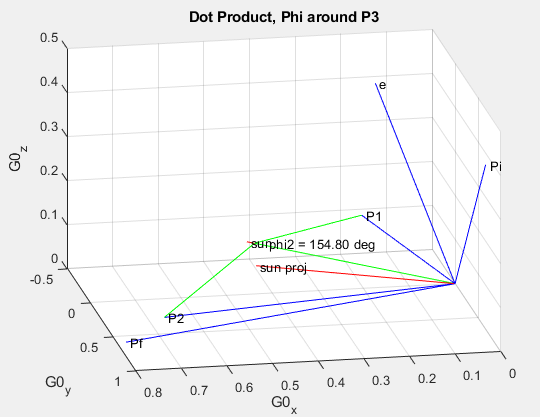
\includegraphics[width=6.25in]{figures/chord_geometry_phi2.png}
				\caption{Chord geometry for finding $\phi_2$}
			\end{figure}
		
		For the first leg of the slew, the spacecraft was rotated around the eigenaxis of the slew plane by $\phi_1$. For the second leg of the slew, the spacecraft was rotated around the sun vector fixed in inertial space by $\phi_2$. For the third leg of the slew, the spacecraft was rotated around the eigenaxis of the slew plane by $\phi_3$. The attitude generated would look like the profile in Figure \ref{fig:phi1_phi2_phi3}. 
		
			\begin{figure}[H]
				\label{fig:phi1_phi2_phi3}
				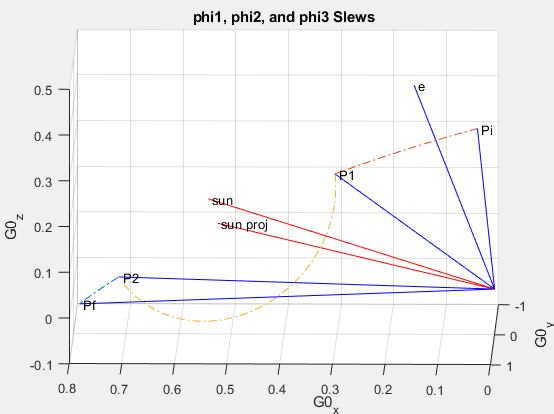
\includegraphics[width=6.25in]{figures/phi1_phi2_phi3.png}
				\caption{Attitude Profile of the Entire Slew}
			\end{figure}
		
		From randomizing the initial, final, and sun position vectors for this simulation, the values of $\phi$ were found and listed in the table below. The angular velocity and acceleration never exceeded the velocity and acceleration constraints for any axis. There is no noise modeled in the actuator system, as the purpose of this simulation was to validate the slewing maneuvers described by the algorithm. 
		
%				\newcommand*{\MyIndent}{\hspace*{0.5cm}}%
				\begin{table}[H]
					\centering
					\caption{Slew Angles $\phi_1$, $\phi_2$, and $\phi_3$}
					\begin{tabular}{llll}
						\toprule
						\midrule
						$\phi$ & 1 & 2 & 3 \\
						\midrule
						Angle (rad) & 0.29 & 2.70 & 0.13 \\
						Angle (deg) & 16.61 & 154.80 & 7.33 \\ 
						\midrule
						\bottomrule
					\end{tabular}%
					\label{tab:FOG_SF}%
				\end{table}%
		

			\begin{figure}[H]
				\label{fig:ang_vel_phi_total}
				\begin{center}
				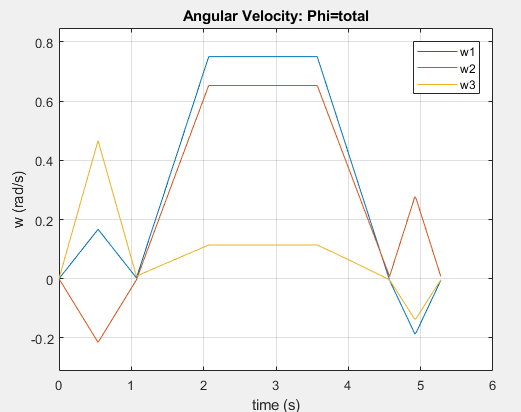
\includegraphics[width=4.5in]{figures/ang_vel_phi_total.png}
				\end{center}
				\caption{Angular Velocity in Spacecraft Frame}
			\end{figure}
		
		
			\begin{figure}[H]
				\label{fig:ang_accel_total}
				\begin{center}
					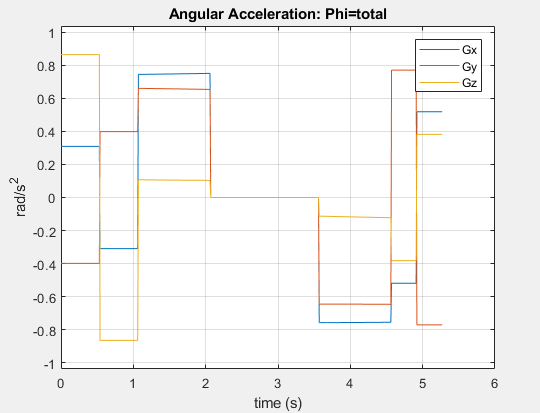
\includegraphics[width=4.5in]{figures/ang_accel_total.png}
				\end{center}
				\caption{Angular Acceleration}
			\end{figure}
		
			\begin{figure}[H]
				\label{fig:quats_phi_total}
				\begin{center}
				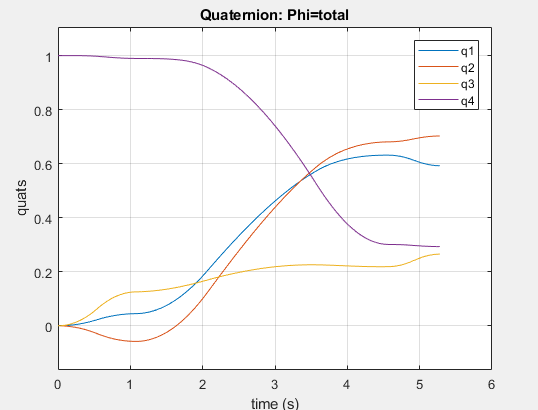
\includegraphics[width=4.5in]{figures/quats_phi_total.png}
				\end{center}
				\caption{Quaternion Attitude}
			\end{figure}
		
			\begin{figure}[H]
				\label{fig:euler_ang_phi_total}
				\begin{center}
				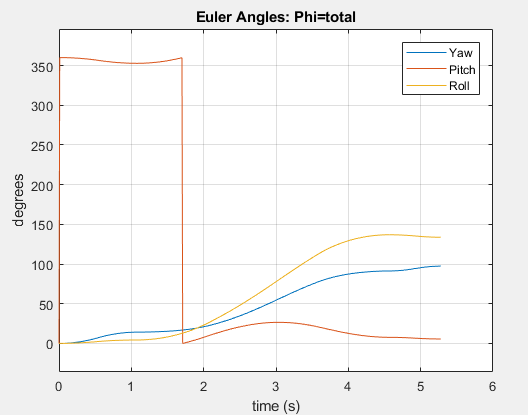
\includegraphics[width=4.5in]{figures/euler_ang_phi_total.png}
				\end{center}
				\caption{Attitude in Euler Angles}
			\end{figure}
		
			\begin{figure}[H]
				\label{fig:torque_total}
				\begin{center}
				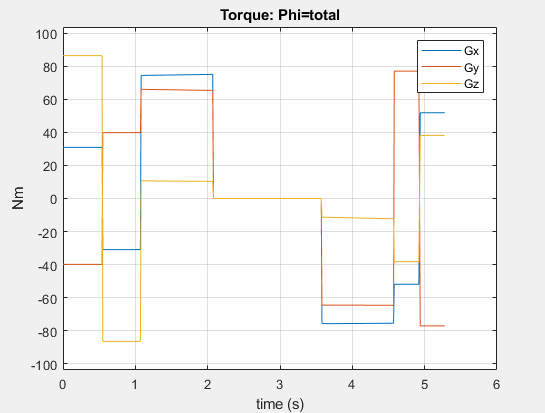
\includegraphics[width=4.5in]{figures/torque_total.png}
				\end{center}
				\caption{Torque Applied from Actuator System}
			\end{figure}
		
			
	
\end{document}
